% !TeX root = f44_shortreport_schmitt_kleinbek.tex
\section{Theoretical Basics}
\subsection{Normal Zeeman effect}
To understand the basics of the Zeeman effect, we first assume that the magnetic moment of an electron $I$ can be sufficiently described by Bohr's atomic model.
According to this model, the electron orbits the atomic nucleus as point mass $m_e$ with velocity $v$ and charge $e$ at a distance $r_\text{B}$, the Bohr radius.\\
Using this approximation, the magnetic moment
\begin{align}
\vec{\mu}_l = \frac{evr}{2}\cdot\vec{n}
\end{align}
is obtained.

%\begin{figure}[ht]
%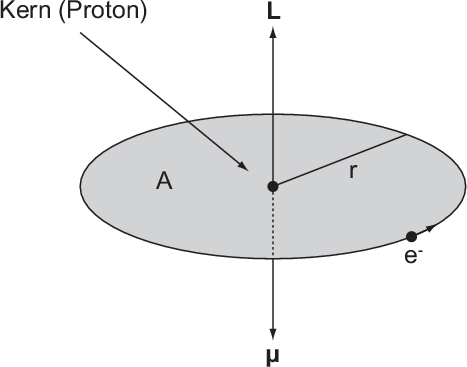
\includegraphics[scale=1]{images//bohrangular.png}
%\caption{Bohr model of an electron with the angular momentum $\vec{L}$ and the magnetic moment $\vec{\mu}$ \cite{ETHZurich}}
%\label{fig:bohrangular}
%\end{figure}

Thus $\vec{n}$ is the normal vector, perpendicular to the disk on which the electron moves.
You can easily see that the magnetic moment resembles the angular momentum of the electron
\begin{align}
\vec{L} = \vec{r} \times \vec{p} = m_e r v \cdot \vec{n}.
\end{align}